\documentclass{fenicscourse}

\begin{document}

\fenicslecture{Lecture 21: Tools for online collaboration}
              {Carl Lundholm, Magne Nordaas}

\begin{frame}
  \frametitle{Introduction}

  Working on projects with other people becomes easier and smoother
  with the right tools.

  \bigskip

  \begin{itemize}
    \item \textbf{Chat applications} \\
      \textbf{\colemph{Slack}}, HipChat, Fleep \\
      \colemph{\url{https://slack.com}}
    \item \textbf{Version control systems (VCSs)} \\
      \textbf{\colemph{Git}}, Mercurial, Subversion \\
      \colemph{\url{https://git-scm.com}}
    \item \textbf{Hosting services for VCS-projects} \\
      \textbf{\colemph{Bitbucket}}, GitHub \\
      \colemph{\url{https://bitbucket.org}}
  \end{itemize}
\end{frame}

\begin{frame}
  \frametitle{Slack}

  Slack is a cloud-based team collaboration tool [Wikipedia].

  \begin{center}
    
\includegraphics[width=0.4\textwidth]{png/slack_logo.png}
  \end{center}

  A nice chat application that is:
  \begin{itemize}
    \item An alternative to email
    \item Well structured for teams
    \item Informal
    \item Quick and easy
    \item Free
  \end{itemize}

  \bigskip

  Homepage: \colemph{\url{https://slack.com}}
\end{frame}

\begin{frame}
  \frametitle{Git: Introduction}

  Git is a command-line based VCS.

  \begin{center}
    
\includegraphics[width=0.3\textwidth]{png/git_logo.png}
  \end{center}

  A tool for managing and tracking different versions of a code.

  \bigskip

  \begin{itemize}
    \item Homepage (downloads for Windows, Linux, Mac OS X) \\
      \colemph{\url{https://git-scm.com}}
    \item The Pro Git book \\
      \colemph{\url{https://git-scm.com/book/en/v2}}
    \item git - the simple guide (downloads and basic commands)\\
      \colemph{\url{http://rogerdudler.github.io/git-guide/}}
  \end{itemize}

\end{frame}

\begin{frame}
  \frametitle{Git: How it works}

  \begin{center}
    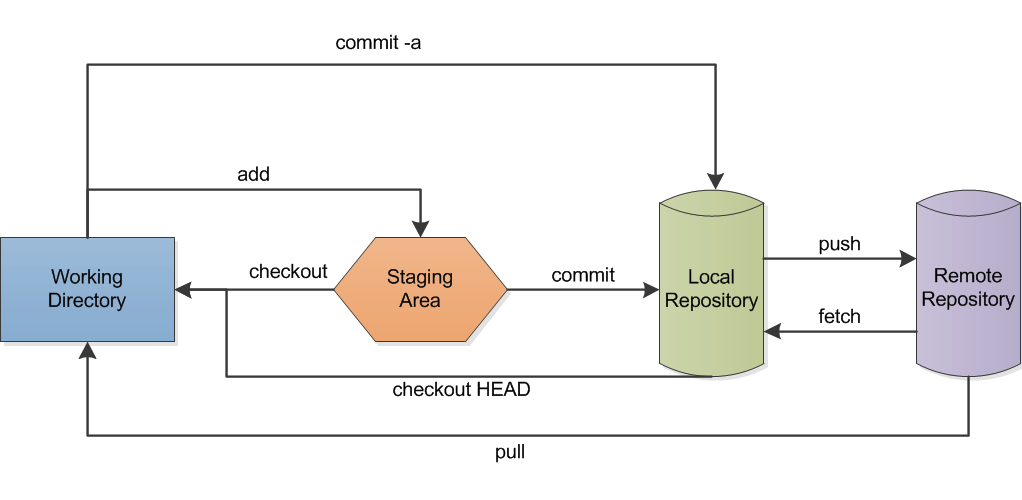
\includegraphics[width=\textwidth]{png/git_flowchart4.png}
  \end{center}

  \begin{itemize}
    \item Working directory - local directory with project files.
     \item Staging area - file with snapshots of project files.
     \item Local repository - local Git directory.
     \item Remote repository - remote Git directory.
  \end{itemize}
\end{frame}

\begin{frame}
  \frametitle{Git: Common commands}

  \begin{itemize}
    \item \texttt{git status} - displays file status.
    \item \texttt{git add} - adds files to staging area.
    \item \texttt{git commit} - commits staged files to local repository.
    \item \texttt{git push} - pushes from local to remote repository.
    \item \texttt{git fetch} - fetches remote to local repository.
    \item \texttt{git merge} - merges local repository with working directory.
    \item \texttt{git pull} - pulls from remote repository directly to
      working directory (= \texttt{git fetch \&\& git merge}).
  \end{itemize}

  \bigskip

  For more commands, type \texttt{git} or \texttt{git help} or see e.g.
  \colemph{\url{https://git-scm.com/docs}} \\
  \colemph{\url{https://confluence.atlassian.com/bitbucketserver/basic-git-commands-776639767.html}}
\end{frame}

\begin{frame}
  \frametitle{Git: Branches and merging}

  \textbf{Branches} are different versions of the code e.g. master (main)
  branch and various feature and test branches.

  \begin{center}
    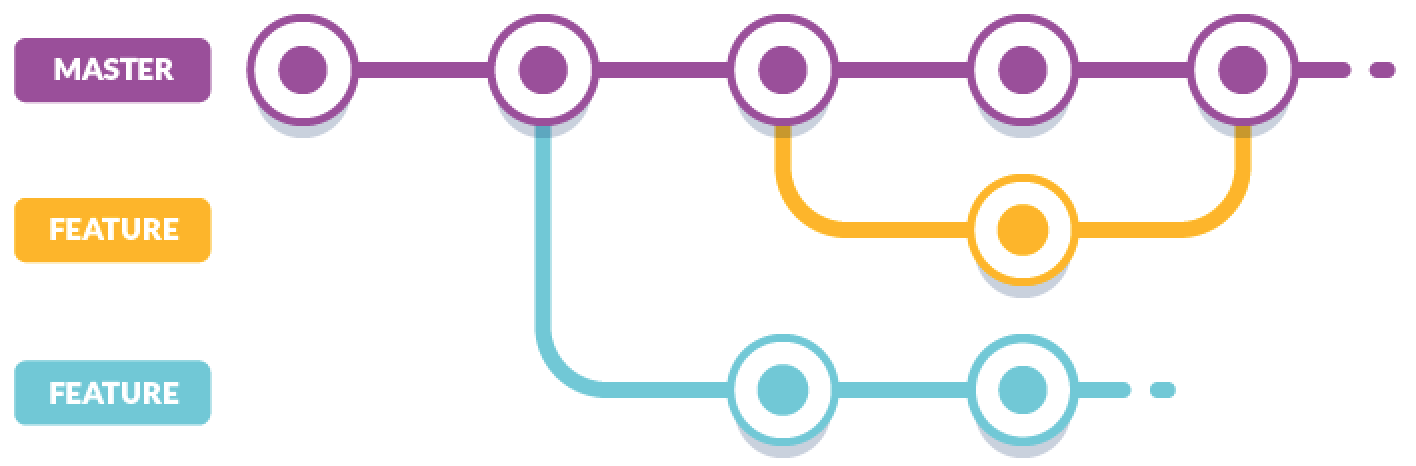
\includegraphics[width=0.7\textwidth]{png/git_branches.png}
  \end{center}

  \textbf{Merging} is joining two branches together.

  \begin{itemize}
  \item  Tips to avoid merge conflicts:
    \begin{enumerate}
      \item Commit often. Better with many small commits than few big ones.
      \item Work on different parts of the code.
    \end{enumerate}
  \item Resolve merge conflicts with \texttt{git mergetool}. There are
    different mergetools e.g. meld and vimdiff.
  \end{itemize}
\end{frame}

\begin{frame}
  \frametitle{Bitbucket}

  Bitbucket is an online hosting service for Git projects.

  \begin{center}
    
\includegraphics[width=0.5\textwidth]{png/bitbucket_logo.png}
  \end{center}

  Git has a command-line user interface (CLI). Bitbucket provides a
  more visual representation of Git projects.

  \bigskip

  Bitbucket is also used by FEniCS developers \colemph{\url{https://bitbucket.org/fenics-project/}}

  \bigskip

  Homepage: \colemph{\url{https://bitbucket.org}}
\end{frame}

\begin{frame}
  \frametitle{Exercise: Using Git and Bitbucket}

  Team up with a partner and practice using Git to push and pull files
  to and from repositories on Bitbucket.

  \bigskip

  \begin{center}
    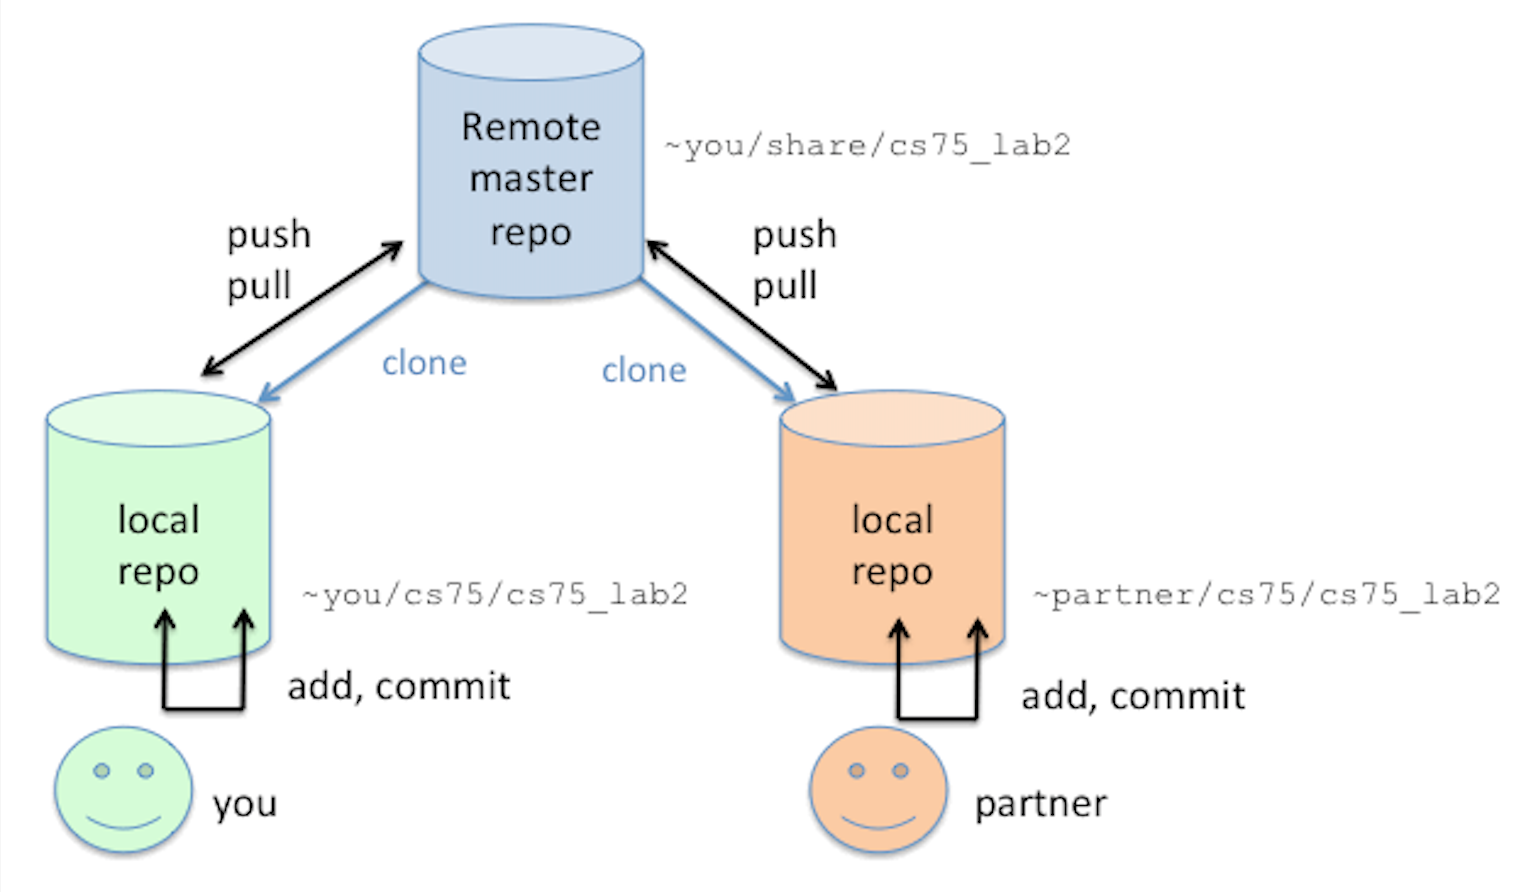
\includegraphics[width=0.7\textwidth]{png/git_repos.png}
  \end{center}
\end{frame}

\begin{frame}
  \frametitle{Exercise: Using Git and Bitbucket (Detailed)}

  Every course member is supposed to:
  \begin{enumerate}
    \item Choose an exercise partner.
    \item Create an account and a remote Git repository on Bitbucket.
    \item Download and install Git.
    \item \texttt{git clone} the remote repository.
    \item Copy a file to the working directory (the folder that was
      created after cloning). \texttt{git add}, \texttt{git commit},
      and \texttt{git push} the file to the remote repository.
    \item Share the repository on Bitbucket with your exercise partner.
    \item \texttt{git clone} the repository you have been invited to.
    \item Modify your partner's file and upload it to your partner's remote repository.
    \item \texttt{git pull} your own updated remote repository.
  \end{enumerate}
\end{frame}


\end{document}
